%============================ PRUEBAS (ENTREGA 2) ===========================
\chapter{Pruebas de validación y seguridad}
\label{cap:pruebas}

\section{Estrategia de pruebas}
La validación combinó \emph{pruebas funcionales} de extremo a extremo (ingesta, análisis, persistencia y registro) con \emph{pruebas de seguridad} centradas en el control de acceso. Las pruebas se ejecutaron mediante un \emph{banco automatizado} en Node.js que levanta instancias aisladas del servidor (sin datos reales), inyecta escaneos y registros simulados por REST y por WebSocket, verifica las respuestas y reinicia el proceso para comprobar la persistencia. El banco reporta cada caso con su resultado observado y una medición de latencia; la totalidad de los casos aquí documentados se superó de forma reproducible (véase la Figura~\ref{fig:consola} en la Sección~\ref{sec:evidencia}).

\section{Casos de prueba funcionales}
La Tabla~\ref{tab:casos} resume los casos ejecutados con su resultado observado.

\begin{table}[H]
\centering
\caption{Casos de prueba funcionales y resultados}
\label{tab:casos}
\footnotesize
\begin{tabularx}{\linewidth}{@{}l X l l@{}}
\toprule
\textbf{ID} & \textbf{Descripción} & \textbf{Esperado} & \textbf{Estado} \\
\midrule
CP01 & Ingesta de escaneo Wi-Fi (3 dispositivos) & \code{received:3} & \textbf{OK} \\
CP02 & Fabricante por OUI (A85C2C, D85D4C) & Apple, TP-Link & \textbf{OK} \\
CP03 & Detección de MAC aleatoria & Marca privacidad & \textbf{OK} \\
CP04 & Evil twin (2 BSSID, SSID "CasaWifi") & Ambos marcados & \textbf{OK} \\
CP05 & Análisis de canal (best/worst/rec.) & Salida coherente & \textbf{OK} \\
CP06 & Serie temporal (muestra por minuto) & Muestras acumuladas & \textbf{OK} \\
CP07 & Persistencia y restauración tras reinicio & Estado recuperado & \textbf{OK} \\
CP08 & Alta de invitado por el portal & \code{success} + total & \textbf{OK} \\
CP09 & Exportación CSV con BOM UTF-8 & CSV con acentos & \textbf{OK} \\
CP10 & Borrado de registros (con sesión) & \code{cleared} & \textbf{OK} \\
\bottomrule
\end{tabularx}
\end{table}

\section{Casos de prueba de seguridad}
Las pruebas de seguridad verificaron que las acciones sensibles exigen las credenciales adecuadas. La Tabla~\ref{tab:seg} presenta los resultados; los códigos de estado HTTP obtenidos confirman el correcto funcionamiento del control de acceso.

\begin{table}[H]
\centering
\caption{Casos de prueba de seguridad (control de acceso)}
\label{tab:seg}
\footnotesize
\begin{tabularx}{\linewidth}{@{}l X c c@{}}
\toprule
\textbf{ID} & \textbf{Escenario} & \textbf{Esperado} & \textbf{Obtenido} \\
\midrule
SEC01 & \code{POST /api/mode} sin token de sesión & 401 & 401 \\
SEC02 & \code{POST /api/mode} con token válido & 200 & 200 \\
SEC03 & \code{GET /api/registrations} sin sesión & 401 & 401 \\
SEC04 & \code{GET /api/registrations} con sesión & 200 & 200 \\
SEC05 & Ingesta con \code{EILOR\_DEVICE\_TOKEN} y sin token & 401 & 401 \\
SEC06 & Ingesta con token de dispositivo correcto & 200 & 200 \\
SEC07 & Login con contraseña incorrecta & 401 & 401 \\
\bottomrule
\end{tabularx}
\end{table}

\section{Análisis de amenazas y mitigaciones}
La Tabla~\ref{tab:amenazas} relaciona las principales amenazas con los controles implementados, siguiendo el enfoque de buenas prácticas de OWASP \parencite{owasp2021}.

\begin{table}[H]
\centering
\caption{Amenazas y controles implementados}
\label{tab:amenazas}
\footnotesize
\begin{tabularx}{\linewidth}{@{}X X@{}}
\toprule
\textbf{Amenaza} & \textbf{Control en EILOR} \\
\midrule
Comandos de control no autorizados & Token de sesión (TTL 24~h) y \code{requireAuth} en rutas de control \\
Inyección de datos falsos por terceros & Token de dispositivo opcional (\code{deviceAuthorized}) en la ingesta \\
Suplantación de red (evil twin) & Detección y marcado de SSID con múltiples BSSID \\
Rastreo por MAC & Detección y señalización de MAC aleatorizadas \\
Exposición del servidor & Publicación por túnel Cloudflare sin puertos entrantes y TLS en el borde \\
Fuga de datos de invitados & Exportación restringida a sesión; minimización de campos recolectados \\
\bottomrule
\end{tabularx}
\end{table}

\section{Métricas de calidad y desempeño observadas}
La Tabla~\ref{tab:metricas} consolida las métricas medidas durante las pruebas.

\begin{table}[H]
\centering
\caption{Métricas de desempeño observadas}
\label{tab:metricas}
\footnotesize
\begin{tabularx}{\linewidth}{@{}X l@{}}
\toprule
\textbf{Métrica} & \textbf{Valor} \\
\midrule
Periodo de ciclo de escaneo & $\sim$3~s \\
Periodo de \emph{heartbeat} & 3~s \\
Umbral de \emph{watchdog} de desconexión & 15~s \\
Frecuencia de muestreo de serie temporal & 1 muestra/min (720 muestras $\approx$ 12~h) \\
Frecuencia de \emph{snapshot} de estado & 30~s \\
Catálogo OUI & 123 prefijos \\
Latencia ingesta $\rightarrow$ \emph{push} (mediana / P95) & 2.5 / 3.2~ms \\
Casos funcionales superados & 10/10 (100\,\%) \\
Casos de seguridad superados & 7/7 (100\,\%) \\
\bottomrule
\end{tabularx}
\end{table}

\section{Evidencia de ejecución}
\label{sec:evidencia}
La Figura~\ref{fig:consola} reproduce la salida del banco automatizado. Además de los casos de las Tablas~\ref{tab:casos} y~\ref{tab:seg}, el banco ejercita rutas adicionales ---registro por WebSocket, rechazo de comandos WebSocket sin sesión, invalidación de token tras \emph{logout} y registro con token de dispositivo erróneo--- alcanzando 20/20 verificaciones superadas.

\begin{figure}[H]
\centering
\setlength{\fboxsep}{0pt}\setlength{\fboxrule}{0.4pt}%
\fcolorbox{gray!45}{white}{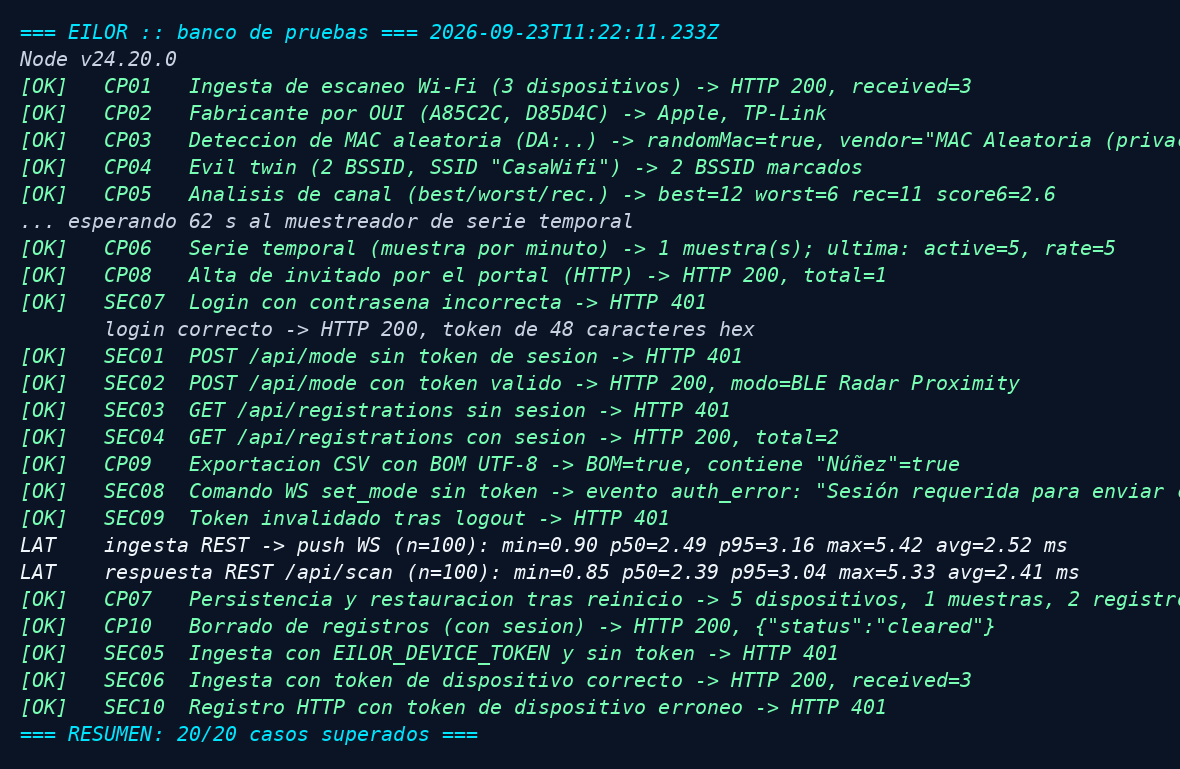
\includegraphics[width=0.98\linewidth]{figuras/cap-consola}}
\caption{Salida de consola del banco de pruebas automatizado: 20/20 casos superados, con los códigos de control de acceso (401/200) y las latencias medidas.}
\label{fig:consola}
\end{figure}
\captura[0.98]{cap-registros}{Registros de invitados visibles en el \emph{dashboard} en tiempo real, con exportación a CSV restringida a la sesión autenticada.}
